\documentclass{standalone}
\usepackage{tikz}
\usetikzlibrary{patterns, positioning}

\begin{document}
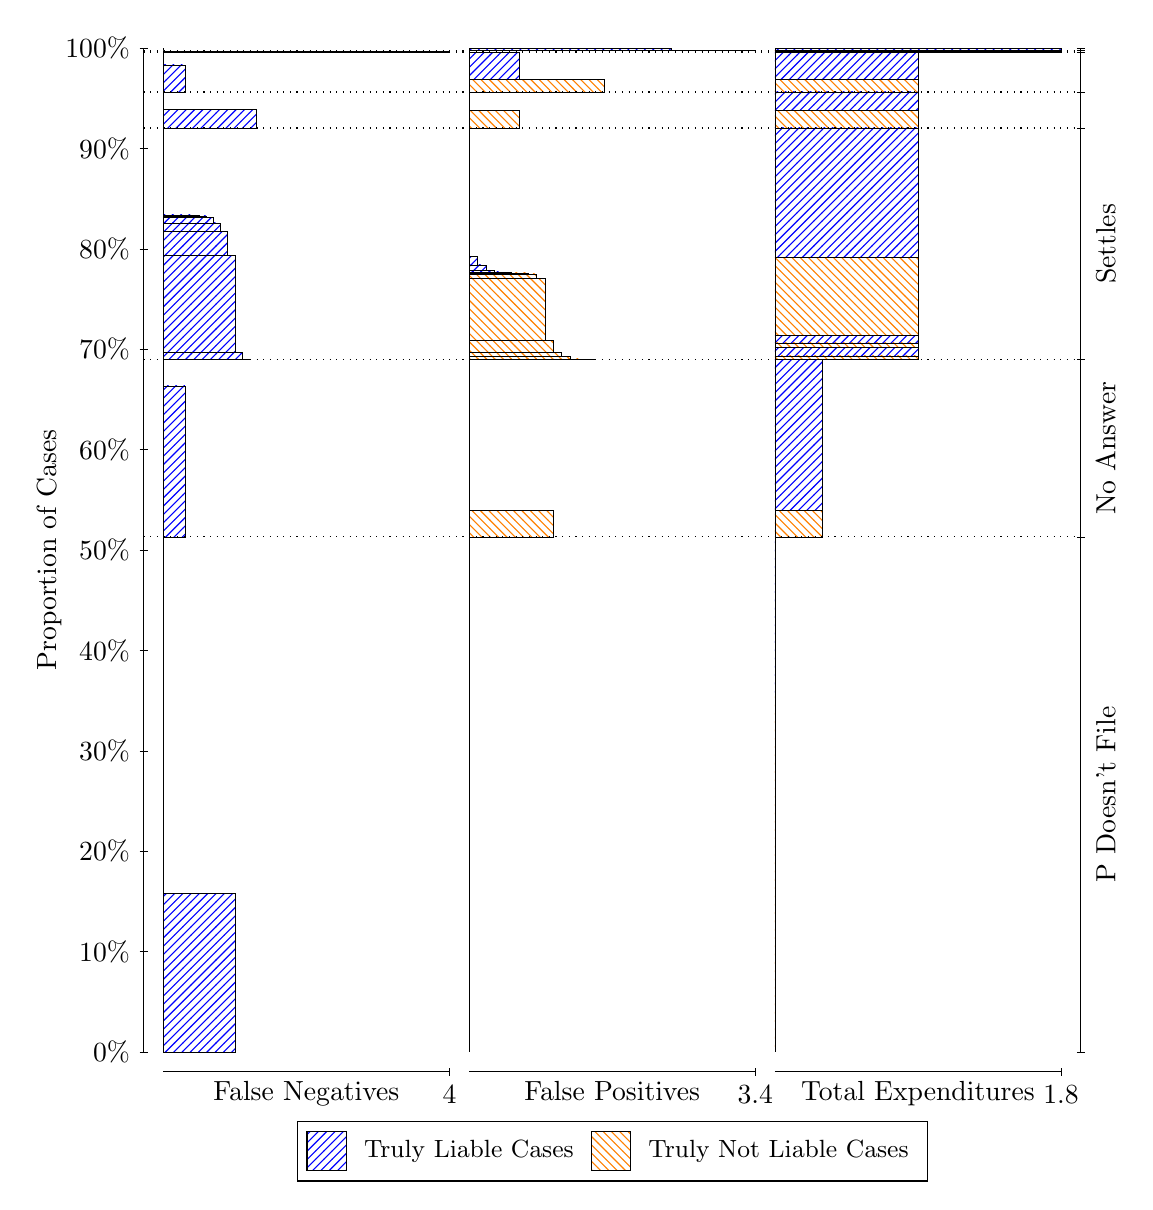
\begin{tikzpicture}
\draw[black, very thin] (1.5,1.75) -- (1.5,14.5);
\node[rotate=90, anchor=center] at (0.3, 8.125) {Proportion of Cases};
\draw[black, very thin] (1.45,1.75) -- (1.55,1.75);
\node[anchor=east] at (1.45, 1.75) {0\%};
\draw[black, very thin] (1.45,3.025) -- (1.55,3.025);
\node[anchor=east] at (1.45, 3.025) {10\%};
\draw[black, very thin] (1.45,4.3) -- (1.55,4.3);
\node[anchor=east] at (1.45, 4.3) {20\%};
\draw[black, very thin] (1.45,5.575) -- (1.55,5.575);
\node[anchor=east] at (1.45, 5.575) {30\%};
\draw[black, very thin] (1.45,6.85) -- (1.55,6.85);
\node[anchor=east] at (1.45, 6.85) {40\%};
\draw[black, very thin] (1.45,8.125) -- (1.55,8.125);
\node[anchor=east] at (1.45, 8.125) {50\%};
\draw[black, very thin] (1.45,9.4) -- (1.55,9.4);
\node[anchor=east] at (1.45, 9.4) {60\%};
\draw[black, very thin] (1.45,10.675) -- (1.55,10.675);
\node[anchor=east] at (1.45, 10.675) {70\%};
\draw[black, very thin] (1.45,11.95) -- (1.55,11.95);
\node[anchor=east] at (1.45, 11.95) {80\%};
\draw[black, very thin] (1.45,13.225) -- (1.55,13.225);
\node[anchor=east] at (1.45, 13.225) {90\%};
\draw[black, very thin] (1.45,14.5) -- (1.55,14.5);
\node[anchor=east] at (1.45, 14.5) {100\%};

\draw[black, very thin] (13.4,1.75) -- (13.4,14.5);
\draw[black, very thin] (13.35,1.75) -- (13.45,1.75);
\node[anchor=west] at (13.35, 1.75) {};
\draw[black, very thin] (13.35,8.2919) -- (13.45,8.2919);
\node[anchor=west] at (13.35, 8.2919) {};
\draw[black, very thin] (13.35,10.541) -- (13.45,10.541);
\node[anchor=west] at (13.35, 10.541) {};
\draw[black, very thin] (13.35,13.485) -- (13.45,13.485);
\node[anchor=west] at (13.35, 13.485) {};
\draw[black, very thin] (13.35,13.942) -- (13.45,13.942);
\node[anchor=west] at (13.35, 13.942) {};
\draw[black, very thin] (13.35,14.449) -- (13.45,14.449);
\node[anchor=west] at (13.35, 14.449) {};
\draw[black, very thin] (13.35,14.468) -- (13.45,14.468);
\node[anchor=west] at (13.35, 14.468) {};
\draw[black, very thin] (13.35,14.5) -- (13.45,14.5);
\node[anchor=west] at (13.35, 14.5) {};

\draw[black, very thin, pattern color=blue, pattern=north east lines] (1.75,1.75) rectangle (2.6583,3.76);
\draw[black, very thin, pattern color=orange, pattern=north west lines] (1.75,3.76) rectangle (1.75,8.2919);
\draw[black, very thin, pattern color=blue, pattern=north east lines] (1.75,8.2919) rectangle (2.0225,10.209);
\draw[black, very thin, pattern color=orange, pattern=north west lines] (1.75,10.209) rectangle (1.75,10.541);
\draw[black, very thin, pattern color=blue, pattern=north east lines] (1.75,10.541) rectangle (2.84,10.549);
\draw[black, very thin, pattern color=blue, pattern=north east lines] (1.75,10.549) rectangle (2.7492,10.636);
\draw[black, very thin, pattern color=blue, pattern=north east lines] (1.75,10.636) rectangle (2.6583,11.865);
\draw[black, very thin, pattern color=blue, pattern=north east lines] (1.75,11.865) rectangle (2.5675,11.87);
\draw[black, very thin, pattern color=blue, pattern=north east lines] (1.75,11.87) rectangle (2.5675,12.174);
\draw[black, very thin, pattern color=blue, pattern=north east lines] (1.75,12.174) rectangle (2.4767,12.28);
\draw[black, very thin, pattern color=blue, pattern=north east lines] (1.75,12.28) rectangle (2.3858,12.353);
\draw[black, very thin, pattern color=blue, pattern=north east lines] (1.75,12.353) rectangle (2.295,12.368);
\draw[black, very thin, pattern color=blue, pattern=north east lines] (1.75,12.368) rectangle (2.2042,12.375);
\draw[black, very thin, pattern color=blue, pattern=north east lines] (1.75,12.375) rectangle (2.1133,12.381);
\draw[black, very thin, pattern color=orange, pattern=north west lines] (1.75,12.381) rectangle (1.75,13.485);
\draw[black, very thin, pattern color=blue, pattern=north east lines] (1.75,13.485) rectangle (2.9308,13.716);
\draw[black, very thin, pattern color=orange, pattern=north west lines] (1.75,13.716) rectangle (1.75,13.942);
\draw[black, very thin, pattern color=blue, pattern=north east lines] (1.75,13.942) rectangle (2.0225,14.287);
\draw[black, very thin, pattern color=orange, pattern=north west lines] (1.75,14.287) rectangle (1.75,14.449);
\draw[black, very thin, pattern color=blue, pattern=north east lines] (1.75,14.449) rectangle (5.3833,14.455);
\draw[black, very thin, pattern color=orange, pattern=north west lines] (1.75,14.455) rectangle (1.75,14.468);
\draw[black, very thin, pattern color=orange, pattern=north west lines] (1.75,14.468) rectangle (1.75,14.474);
\draw[black, very thin, pattern color=blue, pattern=north east lines] (1.75,14.474) rectangle (1.75,14.5);
\draw[black, very thin, pattern color=orange, pattern=north west lines] (5.6333,1.75) rectangle (5.6333,6.2819);
\draw[black, very thin, pattern color=blue, pattern=north east lines] (5.6333,6.2819) rectangle (5.6333,8.2919);
\draw[black, very thin, pattern color=orange, pattern=north west lines] (5.6333,8.2919) rectangle (6.702,8.6234);
\draw[black, very thin, pattern color=blue, pattern=north east lines] (5.6333,8.6234) rectangle (5.6333,10.541);
\draw[black, very thin, pattern color=orange, pattern=north west lines] (5.6333,10.541) rectangle (7.2363,10.543);
\draw[black, very thin, pattern color=orange, pattern=north west lines] (5.6333,10.543) rectangle (7.1294,10.546);
\draw[black, very thin, pattern color=orange, pattern=north west lines] (5.6333,10.546) rectangle (7.0225,10.551);
\draw[black, very thin, pattern color=orange, pattern=north west lines] (5.6333,10.551) rectangle (6.9157,10.587);
\draw[black, very thin, pattern color=orange, pattern=north west lines] (5.6333,10.587) rectangle (6.8088,10.635);
\draw[black, very thin, pattern color=orange, pattern=north west lines] (5.6333,10.635) rectangle (6.702,10.79);
\draw[black, very thin, pattern color=orange, pattern=north west lines] (5.6333,10.79) rectangle (6.5951,11.576);
\draw[black, very thin, pattern color=orange, pattern=north west lines] (5.6333,11.576) rectangle (6.4882,11.633);
\draw[black, very thin, pattern color=orange, pattern=north west lines] (5.6333,11.633) rectangle (6.3814,11.644);
\draw[black, very thin, pattern color=blue, pattern=north east lines] (5.6333,11.644) rectangle (6.1676,11.651);
\draw[black, very thin, pattern color=blue, pattern=north east lines] (5.6333,11.651) rectangle (6.0608,11.657);
\draw[black, very thin, pattern color=blue, pattern=north east lines] (5.6333,11.657) rectangle (5.9539,11.673);
\draw[black, very thin, pattern color=blue, pattern=north east lines] (5.6333,11.673) rectangle (5.8471,11.746);
\draw[black, very thin, pattern color=blue, pattern=north east lines] (5.6333,11.746) rectangle (5.7402,11.852);
\draw[black, very thin, pattern color=blue, pattern=north east lines] (5.6333,11.852) rectangle (5.6333,13.485);
\draw[black, very thin, pattern color=orange, pattern=north west lines] (5.6333,13.485) rectangle (6.2745,13.711);
\draw[black, very thin, pattern color=blue, pattern=north east lines] (5.6333,13.711) rectangle (5.6333,13.942);
\draw[black, very thin, pattern color=orange, pattern=north west lines] (5.6333,13.942) rectangle (7.3431,14.105);
\draw[black, very thin, pattern color=blue, pattern=north east lines] (5.6333,14.105) rectangle (6.2745,14.449);
\draw[black, very thin, pattern color=orange, pattern=north west lines] (5.6333,14.449) rectangle (5.6333,14.463);
\draw[black, very thin, pattern color=blue, pattern=north east lines] (5.6333,14.463) rectangle (5.6333,14.468);
\draw[black, very thin, pattern color=orange, pattern=north west lines] (5.6333,14.468) rectangle (9.2667,14.474);
\draw[black, very thin, pattern color=blue, pattern=north east lines] (5.6333,14.474) rectangle (8.198,14.5);
\draw[black, very thin, pattern color=orange, pattern=north west lines] (9.5167,1.75) rectangle (9.5167,6.2819);
\draw[black, very thin, pattern color=blue, pattern=north east lines] (9.5167,6.2819) rectangle (9.5167,8.2919);
\draw[black, very thin, pattern color=orange, pattern=north west lines] (9.5167,8.2919) rectangle (10.122,8.6234);
\draw[black, very thin, pattern color=blue, pattern=north east lines] (9.5167,8.6234) rectangle (10.122,10.541);
\draw[black, very thin, pattern color=orange, pattern=north west lines] (9.5167,10.541) rectangle (11.333,10.589);
\draw[black, very thin, pattern color=blue, pattern=north east lines] (9.5167,10.589) rectangle (11.333,10.695);
\draw[black, very thin, pattern color=orange, pattern=north west lines] (9.5167,10.695) rectangle (11.333,10.755);
\draw[black, very thin, pattern color=blue, pattern=north east lines] (9.5167,10.755) rectangle (11.333,10.846);
\draw[black, very thin, pattern color=orange, pattern=north west lines] (9.5167,10.846) rectangle (11.333,11.842);
\draw[black, very thin, pattern color=blue, pattern=north east lines] (9.5167,11.842) rectangle (11.333,13.485);
\draw[black, very thin, pattern color=orange, pattern=north west lines] (9.5167,13.485) rectangle (11.333,13.711);
\draw[black, very thin, pattern color=blue, pattern=north east lines] (9.5167,13.711) rectangle (11.333,13.942);
\draw[black, very thin, pattern color=orange, pattern=north west lines] (9.5167,13.942) rectangle (11.333,14.105);
\draw[black, very thin, pattern color=blue, pattern=north east lines] (9.5167,14.105) rectangle (11.333,14.449);
\draw[black, very thin, pattern color=orange, pattern=north west lines] (9.5167,14.449) rectangle (13.15,14.463);
\draw[black, very thin, pattern color=blue, pattern=north east lines] (9.5167,14.463) rectangle (13.15,14.468);
\draw[black, very thin, pattern color=orange, pattern=north west lines] (9.5167,14.468) rectangle (13.15,14.474);
\draw[black, very thin, pattern color=blue, pattern=north east lines] (9.5167,14.474) rectangle (13.15,14.5);
\draw[black, dotted] (1.5,8.2919) -- (13.4,8.2919);
\draw[black, dotted] (1.5,10.541) -- (13.4,10.541);
\draw[black, dotted] (1.5,13.485) -- (13.4,13.485);
\draw[black, dotted] (1.5,13.942) -- (13.4,13.942);
\draw[black, dotted] (1.5,14.449) -- (13.4,14.449);
\draw[black, dotted] (1.5,14.468) -- (13.4,14.468);
\draw[black, very thin] (1.75,1.5) -- (5.3833,1.5);
\node[anchor=north] at (3.5667, 1.5) {False Negatives};
\draw[black, very thin] (5.3833,1.45) -- (5.3833,1.55);
\node[anchor=north] at (5.3833, 1.45) {4};

\draw[black, very thin] (5.6333,1.5) -- (9.2667,1.5);
\node[anchor=north] at (7.45, 1.5) {False Positives};
\draw[black, very thin] (9.2667,1.45) -- (9.2667,1.55);
\node[anchor=north] at (9.2667, 1.45) {3.4};

\draw[black, very thin] (9.5167,1.5) -- (13.15,1.5);
\node[anchor=north] at (11.333, 1.5) {Total Expenditures};
\draw[black, very thin] (13.15,1.45) -- (13.15,1.55);
\node[anchor=north] at (13.15, 1.45) {1.8};

\node[black, centered, rotate=90] at (13.72, 5.0209) {P Doesn't File};
\node[black, centered, rotate=90] at (13.72, 9.4162) {No Answer};
\node[black, centered, rotate=90] at (13.72, 12.013) {Settles};





\draw (7.449999999999999,1.5) node[draw=none] (baseCoordinate) {};
\begin{scope}[align=center]
        \matrix[scale=0.5, draw=black, below=0.5cm of baseCoordinate, nodes={draw}, column sep=0.1cm]{
            \node[rectangle, draw, minimum width=0.5cm, minimum height=0.5cm, pattern=north east lines, pattern color=blue] {}; &
            \node[draw=none, font=\small] (B) {Truly Liable Cases}; &
            \node[rectangle, draw, minimum width=0.5cm, minimum height=0.5cm, pattern=north west lines, pattern color=orange] {}; &
            \node[draw=none, font=\small] (B) {Truly Not Liable Cases}; \\
            };
\end{scope}

\end{tikzpicture}
\end{document}